\documentclass{standalone}
\usepackage{tikz}
\usetikzlibrary{arrows,positioning} 
\usetikzlibrary{fit}



\tikzset{
	%Define standard arrow tip
	>=stealth',
	%Define style for boxes
	punkt/.style={
		circle,
		rounded corners,
		draw=black, very thick,
		text width=2.5em,
		minimum height=1em,
		text centered},
	% Define arrow style
	pil/.style={
		->,
		thick,
		shorten <=2pt,
		shorten >=2pt,}
}

\begin{document}
	
	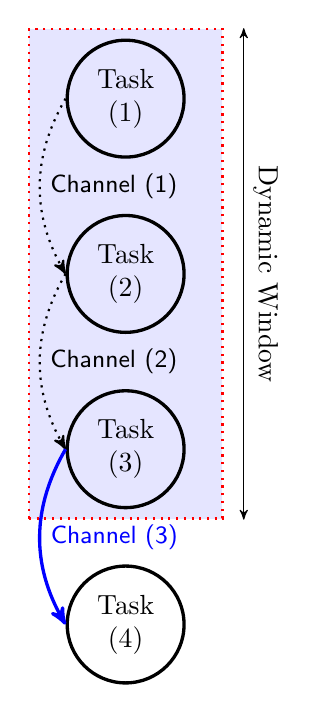
\begin{tikzpicture}[node distance=1cm, auto,]
	
	\pgfdeclarelayer{bg}    % declare background layer
	\pgfsetlayers{bg,main}  % set the order of the layers (main is the standard layer)
	
	\node[punkt] (task1) {Task (1)};
	\node[punkt, below =0.7cm of task1] (task2) {Task (2)};
	\node[punkt, below =0.7cm of task2] (task3) {Task (3)};
	\node[punkt, below =0.7cm of task3] (task4) {Task (4)};
	
	\path[every node/.style={font=\sffamily\small}]
	(task1.west) edge [->, dotted, thick, bend right] node {Channel (1)} (task2.west)
	(task2.west) edge [->, dotted, thick, bend right] node {Channel (2)} (task3.west)
	(task3.west) edge [->, very thick, blue, bend right] node {Channel (3)} (task4.west);
	
	\begin{pgfonlayer}{bg}    % select the background layer
		\node[draw,thick,dotted,red,minimum width=7em, fill=blue!10, fit=(task1) (task2) (task3)] (Virtualized) {};
		\draw[<->] ([xshift=1.5cm]Virtualized.north) --node[sloped, anchor=south] {Dynamic Window} ([xshift=1.5cm]Virtualized.south);
	\end{pgfonlayer}
	
	\end{tikzpicture}
	
\end{document}